\documentclass[12pt]{article}
\author{GUILBERT Augustin, MARTINANT Valentin, OZDEMIR Serdar} 
\date{\today}
\title{\textsc{\textbf{Compression d'images}}}
\renewcommand{\baselinestretch}{1.2}
\usepackage{graphicx}
\usepackage[utf8]{inputenc} %accent
\usepackage[T1]{fontenc} %accent
\usepackage[frenchb]{babel} % choix de la langue 
\usepackage{graphicx} %inclure des images(PNG,JPG,PDF)
\usepackage{amsmath,amssymb}
\usepackage[top=2.5cm,bottom=2.5cm,left=2.5cm,right=2.5cm]{geometry} 
\usepackage{fancyhdr}
\usepackage{caption}
\pagestyle{fancy} 
\lfoot{TIPE Compression d'images} 
\rfoot{Lycée Blaise Pascal 2017-2018} 

\renewcommand{\footrulewidth}{0.8pt}

\begin{document}
\maketitle
\newpage
\tableofcontents
\newpage
\section{Objectifs et types de compression d'images}	
Les images peuvent être codées « naïvement » : il s’agit d’enregistrer une matrice contenant pour chaque pixel, la valeur de celui-ci s’il s’agit d’une image en noir et blanc, les valeurs rouge, verte et bleues si c’est une image en couleur. Ce format est simple à mettre en œuvre et facile à décoder, cependant il est très gourmand en stockage.  Par exemple pour image couleur de taille 500*500 (taille moyenne), il faut près de 75000 octets soit 600000bits ! Ce qui peut s’avérer problématique pour le stockage de grandes quantités d’images, mais aussi lors de transferts. C’est pourquoi il est intéressant de compresser les images, c’est-à-dire diminuer leur poids. Deux types de compression se présentent à l’utilisateur.
D’une part, la compression sans perte, qui permet de conserver une netteté des traits irréprochable. Cette compression est utilisée pour des images nécessitant une très grande précision, tel que les schémas, les dessins techniques ou les balayages médicaux.
D’autre part, la compression avec perte privilégie par définition l’économie de poids à la qualité. Ce qui est utile dans le cas de transmission bas débit, ou pour un stockage de masse d’images, cependant la qualité de l’image est dégradée. Le format JEPG (Joint Photographic Expert Group) s’avère être un bon compromis entre une qualité d’image très correcte et une bonne compression. La compression JPEG s’appuie sur la DCT (Discret Cosinus Transform).
Nous avons réalisé à l’aide du logiciel de programmation Python une compression de type JPEG.


\newpage
\section{Compression JPEG}
La compression JPEG permet une bonne qualité car elle utilise la DCT. En effet, la DCT permet de traduire une information spatiale en une information fréquentielle. Les variations rapides d’intensités, traduites pas les hautes fréquences étant rares, et l’œil humain les percevant mal, elles sont supprimées au cours de la compression. Une image à laquelle on applique la compression JPEG suit le traitement suivant.
\paragraph{}
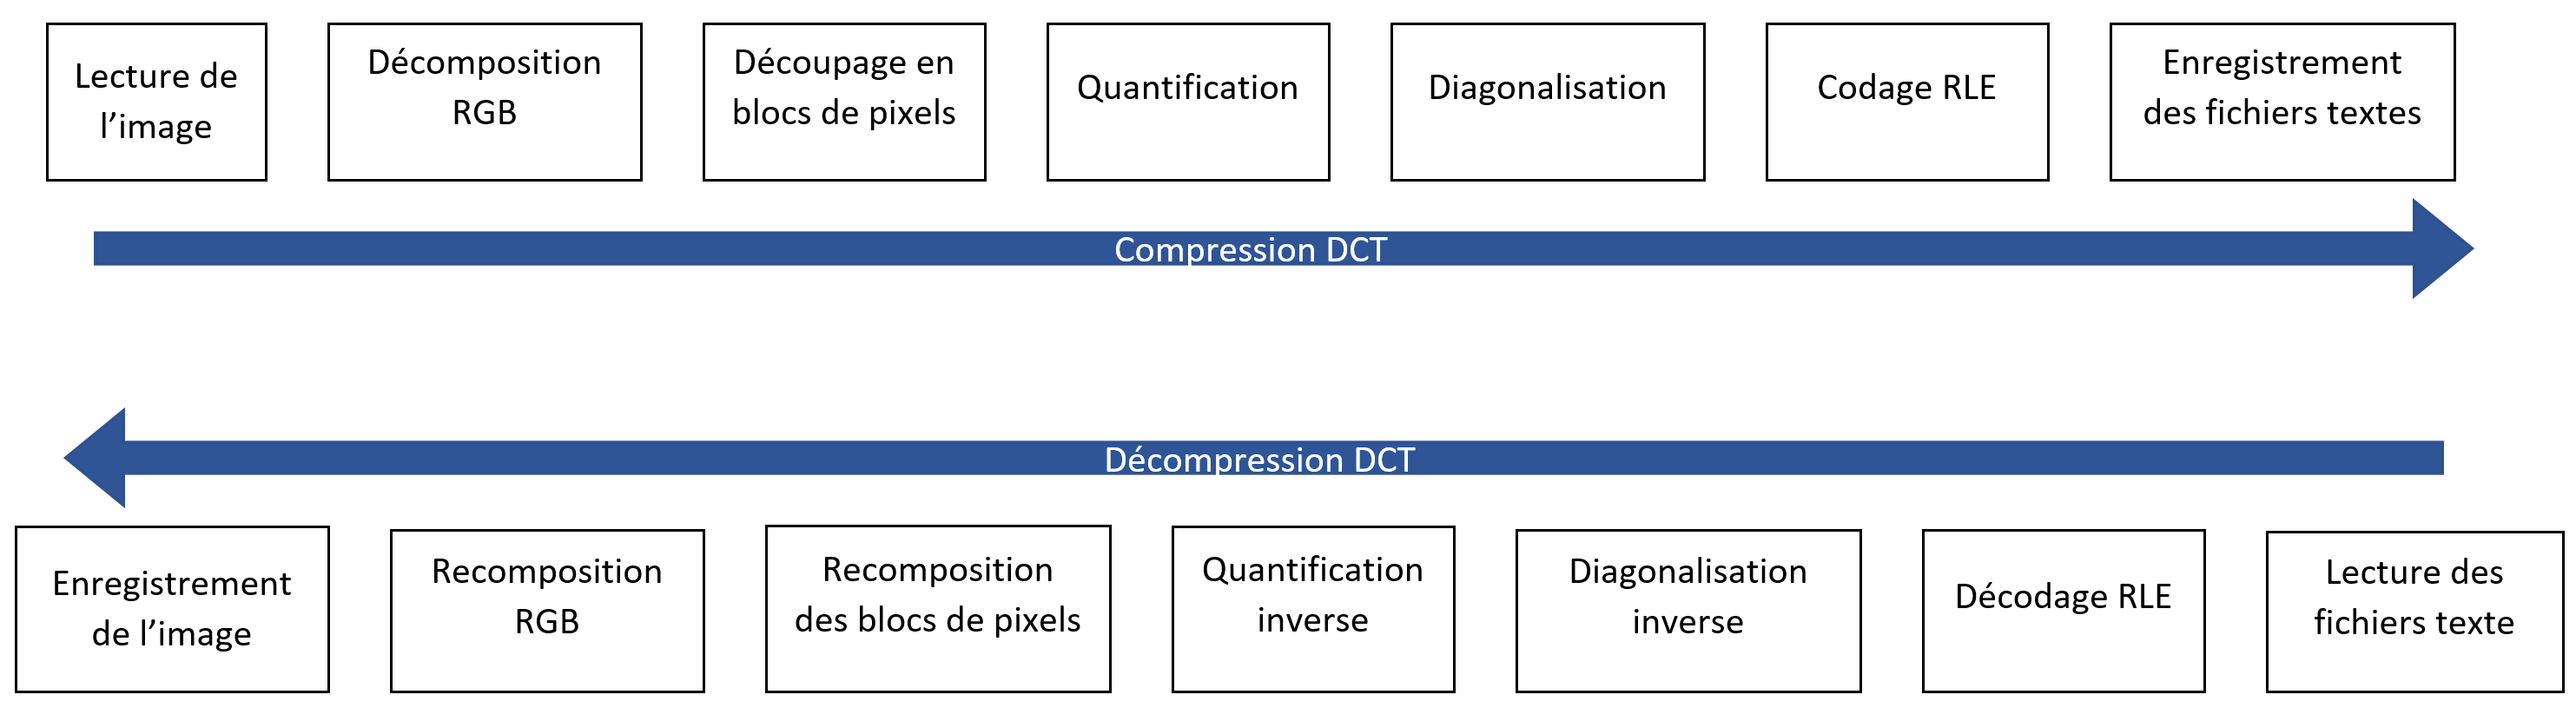
\includegraphics[scale=0.2]{/Users/guilbertaugustin/Desktop/schema_dct.png} %scale pour augmenter ou diminuer proportionnellement la hauteur et largeur de l'image
\paragraph{}
La première étape est la lecture de l’image qui consiste à la convertir en une matrice de dimension 3 (longueur, largeur, nombre de couleurs). Cette étape est suivie dans le cas d’une image en couleur par la décomposition de cette matrice en trois matrices contenant chacune les valeurs du pixel pour une couleur donnée. Il faut ensuite découper cette matrice en blocs carrés de 8 coefficients. Cette opération peut nécessiter le rajout de lignes et de colonnes si le nombre de pixel d’une dimension n’est pas un multiple de 8, les colonnes et lignes rajoutées sont alors des copies de la dernière ligne ou colonne propre à l’image, car elles n’interfèrent pas dans la DCT. Ces blocs de matrices subissent alors un changement de base, permettant de faire apparaître les variations d’intensité sous forme de fréquences. La matrice de passage d’une base à l’autre est la suivante:
\paragraph{}
\begin{center}
$Q=
\begin{Bmatrix}

.3536& .3536& .3536& .3536& .3536& .3536& .3536& .3536 \\
.4904& .4157& .2778& .0975& -.0975& -.2778& -.4157& -.4904 \\
.4619& .1913& -.1913& -.4619& -.4619& -.1913& .1913& .4619 \\
.4157& -.0975& -.4904& -.2778 & .2778& .4904& .0975& -.4157 \\
.3536& -.3536& -.3536& .3536& .3536& -.3536& -.3536& .3536 \\
.2778& -.4904& .0975& .4157& -.4157& -.0975& .4904& -.2778 \\
.1913& -.4619& .4619& -.1913& -.1913& .4619& -.4619& .1913 \\
.0975& -.2778& .4157& -.4904& .4904& -.4157& .2778& -.0975 \\

\end{Bmatrix}
$
\end{center}

\paragraph{}

Ce qui correspond à la formule suivante:
\begin{center}
$Q(i)(j)=
\begin{Bmatrix}
\cfrac{1}{\sqrt{2N}}  \qquad if \quad i=0 \\
\sqrt{\cfrac{2}{N}} \: cos\biggl[\cfrac{2*j+1}{2N}\biggr] \qquad if \quad i>0 \\
\end{Bmatrix}
$
\end{center}
On réalise alors le changement de base suivant la formule suivante: Q.M.Q\up{-1}, le changement de base est équivalent à réaliser cette opération qui donnera une matrice semblable:
\begin{equation*} 
C(i)(j)=\cfrac{1}{\sqrt{2N}} \biggl[\sum_{1\leq x\leq N-1} \sum_{1\leq y\leq N-1} p(x,y) \cos{\biggl[\cfrac{(2x+1) i \Pi}{2N}}\biggr] \cos{\biggl[\cfrac{(2y+1) j \Pi}{2N}}\biggr]\biggr]
\end{equation*}


 Arrive alors l’étape de la quantification qui consiste à diviser les coefficients de l’image par ceux d’une matrice de quantification, permettant de ne conserver que les coefficients les plus importants : 
				%Matrice de quantification
La Matrice ainsi obtenue est alors diagonalisée, c’est-à-dire qu’elle la transforme en liste en la parcourant de la manière suivante :
			%Schéma de la diagonalisation
Cette liste contenant beaucoup de 0 consécutifs, elle subit une RLE (Run-Lenth Encoding), qui consiste à indiquer le nombre de coefficients de même valeur consécutifs et la valeur de ce coefficient. Enfin, ces listes sont enregistrées en tant que fichiers textes et représentent l’image une fois compressée.

La décompression suit le chemins inverse. Tout d’abord, une fonction lit et transforme en liste les fichiers textes contenant l’image compressée, puis ces listes subissent une RLE inverse permettant d’obtenir 64 coefficients. On applique ensuite une diagonalisation inverse, qui consiste à reconstruire une matrice à partir de la liste obtenue. Les coefficients de la matrice sont ensuite multipliés par les coefficients de la matrice de quantification, puis on réalise un changement de base de la matrice dans la base canonique. Les blocs de 64 pixels sont alors rassemblés, puis les colonnes et lignes rajoutées sont supprimées afin de donner à la matrice les dimensions de l’image d’origine. Enfin, dans le cas échéant, les matrices des différentes couleurs sont assemblées puis cette matrice finale est enregistrée au format image pour donner une image finale de même taille que l’image de départ.






\captionsetup{labelformat=empty}
\begin{table}[h]
\begin{center}
\begin{tabular}{|p{2,5cm}|p{3cm}|p{3,3cm}|p{2,5cm}|}
\hline
\centering Niveau de compression&\centering Taille originale (en Mo)&\centering Taille compressée (en Mo)&\centering Taux de compression\tabularnewline%\centering permet de centrer le contenue de la cellule suiante, il faut alors utiliser \tabularnawline pour sauter la ligne car \\ est désactivé
\hline
\centering 10&\centering 6,22&\centering 1,08&\centering 5,7\tabularnewline
\hline
\centering 20&\centering 6,22&\centering 1,26&\centering 4,9\tabularnewline
\hline
\centering 30&\centering 6,22&\centering 1,44&\centering 4,3\tabularnewline
\hline
\centering 40&\centering 6,22&\centering 1,60&\centering 3,9\tabularnewline
\hline
\centering 50&\centering 6,22&\centering 1,76&\centering 3,5\tabularnewline
\hline
\centering 60&\centering 6,22&\centering 1,90&\centering 3,3\tabularnewline
\hline
\centering 70&\centering 6,22&\centering 2,14&\centering 2,9\tabularnewline
\hline
\centering 80&\centering 6,22&\centering 2,56&\centering 2,4\tabularnewline
\hline
\centering 90&\centering 6,22&\centering 3,39&\centering 1,8\tabularnewline
\hline

\end{tabular}
\end{center}
\caption{Taux de compression en fonction du niveau de quantification choisi}
\end{table}

\

\end{document}
